\documentclass[10pt]{article}
%Project write-up
\usepackage{titlesec}	%To show title on the top
%\titleformat*{\section}{\Large\bfseries}
%\titleformat*{\subsection}{\Large\bfseries}
%\titleformat*{\subsubsection}{\large\bfseries}
%\titleformat*{\paragraph}{\large\bfseries}
%\titleformat*{\subparagraph}{\large\bfseries}
\usepackage{natbib}
\bibliographystyle{unsrtnat}

\usepackage{booktabs}	%used for modifying tables
\usepackage{float}	%controling floating objects like tables, figures...
\floatstyle{plaintop}	%?
\restylefloat{table}	%?

\usepackage{geometry}                		% See geometry.pdf to learn the layout options. There are lots.
\geometry{letterpaper}                   		% ... or a4paper or a5paper or ... 

\usepackage{caption}
\usepackage{graphicx}				% Use pdf, png, jpg, or epså€ with pdflatex; use eps in DVI mode	

\usepackage{amssymb}	%maths package
\usepackage{physics}	
\usepackage{IEEEtrantools}

\author{Ananya Bijaya}
\date{October 15, 2018}
\title{\vspace{-1.5cm}           
Dynamic response of a simply supported beam subject to a transient concentrated load at the center}

\begin{document}
%\tableofcontents
\maketitle
\section*{Problem Description}
A simply supported beam, as shown in figure \ref{fig:ssb}, is loaded with a concentrated load at the center; the load is removed after the beam attains the deformed configuration. The response of the beam is required to be calculated for 5 seconds.\newline

\noindent%
\begin{figure}[h!]
	\centering
	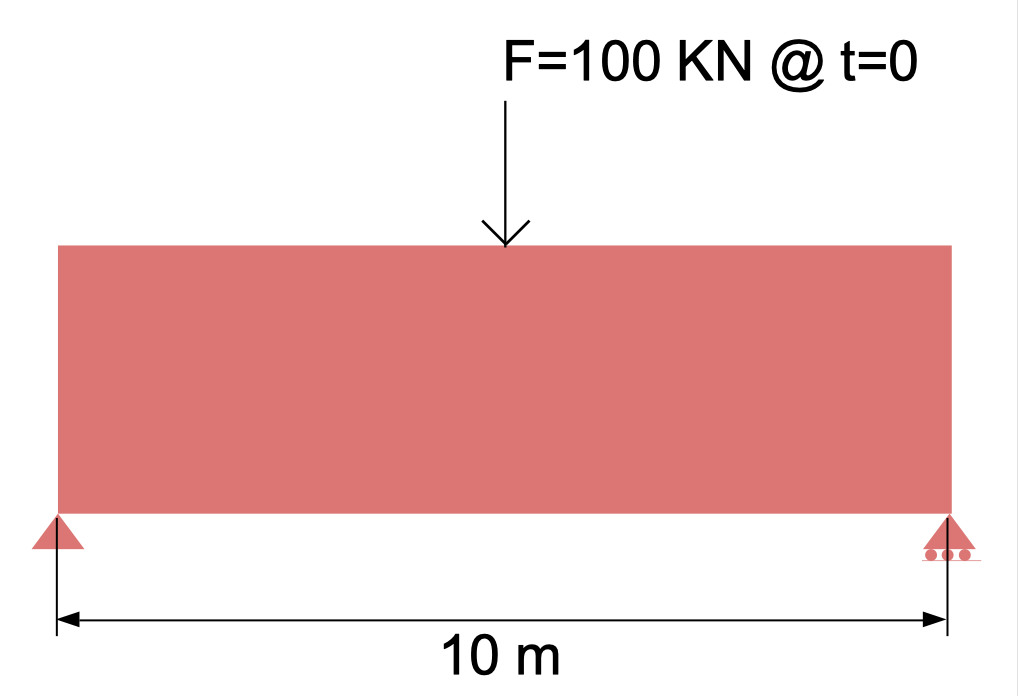
\includegraphics[scale=.25]{ProbDef_rev.png}
	\caption{Schematic of the problem}
	\label{fig:ssb}
\end{figure}
Given: \\
L=10 m \\
A=400 $\times$ 400$\quad mm^2$ \\
E=200 GPa \\
$\rho=7860 \ kg/m^3$\\
F(t=0)=100 KN  \\
\begin{flushleft}
The response of the beam can written in the PDE form as:
\end{flushleft}

\begin{align}
	EI\pdv[4]{w(x,t)}{x}+\rho A\pdv[2]{w(x,t)}{t}=0
\end{align}

Boundary Conditions
\begin{IEEEeqnarray}{lCl} 
	w(x=0,t) & = & 0 \\
	w(x=10,t) & = & 0 \\
	\pdv[2]{w(x=0,t)}{x} & = & 0 \\
	\pdv[2]{w(x=10,t)}{x} & = & 0 
	\end{IEEEeqnarray}

Inital Values \newline
\begin{align}
u(x,t=0)=\frac{Wx}{12EI} \bigg(\frac{3L^2}{4}-x^2\bigg) \\
\pdv{w(x,t=0)}{t}=0
\end{align}

Solution \newline
\begin{IEEEeqnarray}{l}
For\quad 1\leq i\leq n \quad and \quad 1\leq m\leq T\nonumber\\[3pt]
\textit{where: i denotes space and m denotes time} \nonumber\\[3pt]
\rho A \pdv[2]{w}{t}=-EI\pdv[4]{w(x,t)}{x} \nonumber\\[3pt]
\pdv[2]{w}{t}=\frac{w^{m+1}_{i}-2w^m_i+w^{m-1}_i}{\Delta t^2}\nonumber\\[3pt]
\pdv[4]{w}{x}=\frac{w^m_{i-2}-4w^4_{i-1}+6w^m_i-4w^m_{i+1}+w^m_{i+2}}{\Delta x^4}\nonumber\\[3pt]
\frac{w^{m+1}_i-2w^m_i+w^{m-1}_i}{\Delta t^2}=-\frac{EI}{\Delta x^4 \rho A}\Big(w^m_{m-2}-4w^m_{i-1}+6w^m_i-4w^m_{i+1}+w^m_{i+2}\Big) \nonumber\\[3pt] 
w^{m+1}_i=-\frac{EI\Delta t^2}{\Delta x^4 \rho A}\Big(w^m_{i-2}-4w^m_{i-1}+6w^m_i-4w^m_{i+1}+w^m_{i+2}\Big)+2w^m_i-w^{m-1}_i \\[3pt]
\textit{For first time step; Putting m=2}\nonumber\\
\pdv{w}{t}\Big|_{m=1}=\frac{w^1_i-w^{0}_i}{\Delta t}\nonumber \\[3pt]
w^{0}_i=w^1_i-\Delta{t}\pdv{w}{t}\Big|_{m=1}=w_i^1 \nonumber\\[3pt]
\textit{Introducing boundary values in the space derivative in order to get response at i=2 and i=n-1} \nonumber\\[3pt]
\pdv[2]{w}{x}\Big|_i=\frac{w^m_{i+1}-2w^m_i+w^m_{i-1}}{{\Delta x}^2} \nonumber\\[3pt]
\textit{Putting i=1} \nonumber\\[3pt]
w^m_{0}={\Delta x}^2\pdv[2]{w}{x}\Big|_{i=1}+2w^m_1-w^m_{2}=2w^m_1-w^m_{2} \\[3pt]
\textit{Putting i=n} \nonumber\\[3pt]
w^m_{n+1}={\Delta x}^2\pdv[2]{w}{x}\Big|_{i=n}+2w^m_n-w^m_{n-1}=2w^m_n-w^m_{n-1}
\end{IEEEeqnarray}
%\par\noindent\rule{\textwidth}{0.4pt}

For obtaing stable solution $\frac{K\Delta t^2}{\Delta x^4}$ is taken less than 0.25
\begin{IEEEeqnarray*}{l} 
K=\frac{EI}{\rho A}=3.39\times10^5\\[3pt] 
\Delta t=4.0e^{-05} \quad \Delta x=0.217\\[3pt]
\frac{K \Delta t^2}{\Delta x^4}=0.2431
\end{IEEEeqnarray*}

	 
\begin{figure}[h!]
	\centering
	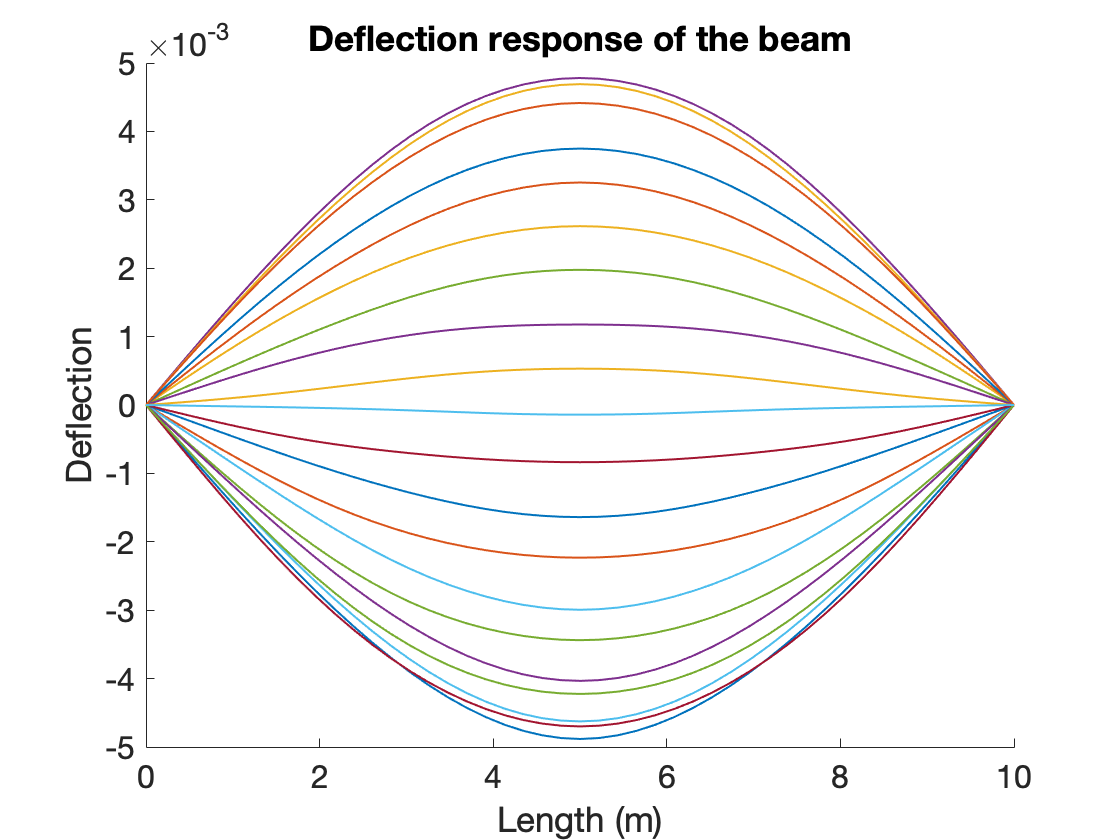
\includegraphics[scale=.25]{Response.png}
	\caption{Response plotted at 0.2 sec intervals}
	\label{Response}
\end{figure}



%\medskip
%\bibliography{research_log_ref}
\end{document}